\begin{figure}[!h]
\centering
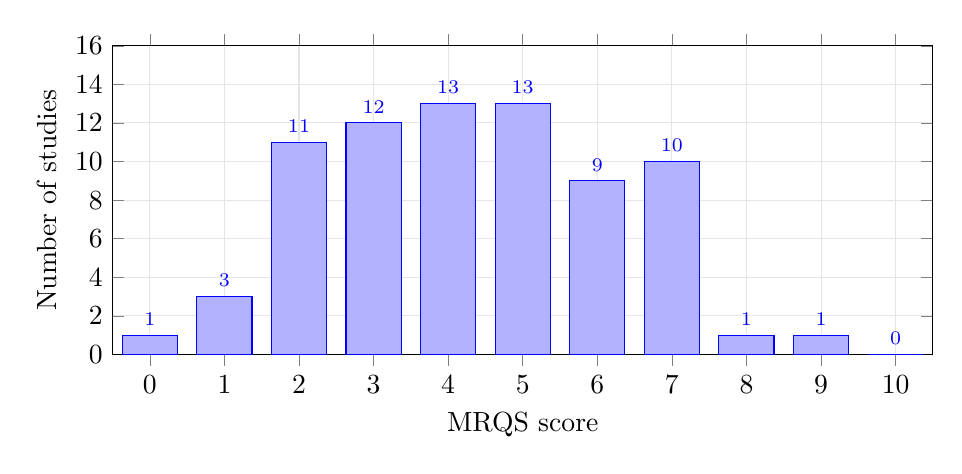
\begin{tikzpicture}
\begin{axis}[
    ybar,
    width=12cm,
    height=5.5cm,
    xlabel={MRQS score},
    ylabel={Number of studies},
    ymin=0, ymax=16,
    xmin=-0.5, xmax=10.5,
    xtick={0,1,2,3,4,5,6,7,8,9,10},
    ytick={0,2,4,6,8,10,12,14,16},
    grid=major,
    grid style={gray!20},
    bar width=0.7cm,
    nodes near coords,
    nodes near coords style={font=\scriptsize, anchor=south},
    every axis plot/.append style={fill=blue!50, draw=blue!70!black},
]
\addplot coordinates {
    (0,1) (1,3) (2,11) (3,12) (4,13) (5,13) (6,9) (7,10) (8,1) (9,1) (10,0)
};
% Modal cluster annotation
\draw[decorate, decoration={brace, amplitude=5pt, raise=22pt}, thick, red!70!black]
    (axis cs:3.6,13) -- (axis cs:5.4,13)
    node[midway, above=27pt, font=\scriptsize, text=red!70!black] {35.2\%};
\end{axis}
\end{tikzpicture}
\caption{Distribution of MRQS scores across 74 included studies. The modal cluster at scores 4--5 accounts for 26 studies (35.2\%). No study achieved the maximum score of 10.}
\label{fig:mrqs-distribution}
\end{figure}
